\chapter{Methodology}
\label{ch:methodology}

The purpose of this work is to categorize medical words according to whether they can be understood or not by non-specialized people, using features obtained with deep learning methods. The manual annotations of these words described in the previous chapter provide the reference data. The proposed method includes three steps: 
\begin{enumerate}
    \item calculation of NLP features associated with the annotated words;
    \item training a machine learning model for word classification;
    \item evaluation of classification quality using cross-validation.
\end{enumerate}
%
In this research we want to provide answers to the following questions:
\begin{enumerate}
    \item Which feature set distinguishes better between understandable and non-understandable medical words?
    \item Why one feature set categorizes better than another?
    \item Do classifiers built on the considered feature sets generalize well? 
\end{enumerate}


\section{Feature sets}
\subsection{Standard NLP features}
\label{sec:standard-features}
We will refer to the previously used NLP features  \citep{Grabar-PITR2014} as \textit{"standard features"} opposed to two kinds of \textit{"embeddings"} described in the next subsection. The standard features include 24 linguistic and extra-linguistic features related to general and specialized languages. The features are computed automatically and can be grouped into ten classes: 

\begin{itemize}
\item {\it Syntactic categories.}  Syntactic categories and lemmas are
  computed by TreeTagger \citep{Schmid-1994} and then checked by FLEMM
  \citep{Namer-TAL2000}.  The syntactic categories are assigned to words within the context of their terms.  If a given word receives more than one category, the most frequent one is kept as a feature.
  Among the main categories, we find for instance nouns, adjectives,  proper names, verbs, and abbreviations.
\item {\it Presence of words in reference lexica.} Two
  reference lexica of the French language were used:
  TLFi\footnote{\url{http://www.atilf.fr/}} and {\it lexique.org}\footnote{\url{http://www.lexique.org/}}. TLFi is a dictionary of the French language covering XIX and XX
  centuries. It contains almost 100,000 entries. {\it lexique.org} is a lexicon created for psycholinguistic experiments. It contains over
  135,000 entries, among which inflectional forms of verbs, adjectives, and nouns. It contains almost 35,000 lemmas.
\item {\it Frequency of words through a non-specialized search
    engine.} For each word, a query to Google search engine was sent in order to find out the frequency of the word attested on the web.
\item {\it Frequency of words in the medical terminology.} The frequency of words in the medical terminology Snomed International was computed.
\item {\it Number and types of semantic categories associated with words.} The information on the semantic categories of
  Snomed International was used.
\item {\it Length of words in a number of their characters and syllables.} For each word, the number of its characters and syllables was computed.
\item {\it Number of bases and affixes.} Each lemma was analyzed by the morphological analyzer D\'erif \citep{Namer-AMIA2004}, adapted to the treatment of medical words. It performs the decomposition of lemmas into bases and affixes known in its database, and it also provides a semantic explanation of the analyzed lexemes. The morphological decomposition information (number of affixes and bases) was exploited.
\item {\it Initial and final substrings of the words.} Initial and final substrings of different length, from three to five characters, were computed.
\item {\it Number and percentage of consonants, vowels and other
    characters.} The number and the percentage of consonants, vowels and other characters (i.e., hyphen, apostrophe,
  comas) was computed.
\item {\it Classical readability scores.} Two classical readability measures were applied: Flesch \citep{Flesch1948} and its variant Flesch-Kincaid \citep{Kincaid-1975}. Such measures are typically used for evaluating the difficulty level of a text. They exploit surface
  characteristics of words (number of characters and/or syllables) and normalize these values with specifically designed coefficients.
\end{itemize}


\subsection{FastText word embeddings usage}

FastText word embeddings (described in section \ref{sec:fasttext}) are a good choice for getting word features in difficulty detection task because they are able to use words' morphological information and generalize over it. The fact that word embeddings capture context and morphological information leads to the hypothesis that incorporating this information as features will improve classification accuracy for our specific problem. 

We found out that FastText word embeddings trained on Wikipedia and Common Crawl\footnote{\url{http://commoncrawl.org/}} texts have a quite large portion of \textit{known} (learned) words from our dataset.
According to our analysis, 44.26\% (13,118 out of 29,641) medical words in the dataset and 56.00\% (16,598 out of 29,641) lowercased medical words in the dataset were used for training of the currently published FastText\footnote{\url{https://fasttext.cc}} model for French.

\subsection{French RNN Medical Understandability Text Embeddings (FrnnMUTE)}
\label{sec:frnnmute-learning}

According to the general functionality of RNN expressed in \ref{sec:rnn}, the final hidden state aggregates the information about the whole input sequence. This idea is frequently used to receive hidden representations of sequences. Sequence-to-sequence (seq2seq) models are a well-known example of how this idea works in practice \citep{Sutskever-NIPS2014}. Such models consist of two parts: an \textit{encoder} is an RNN which encodes input sequence into a representation in hidden space (which is also called \textit{thought vector}), and a \textit{decoder} which generates a new sequence out of the hidden representations (fig. \ref{fig:seq2seq}). 

\begin{figure}[h]
    \centering
    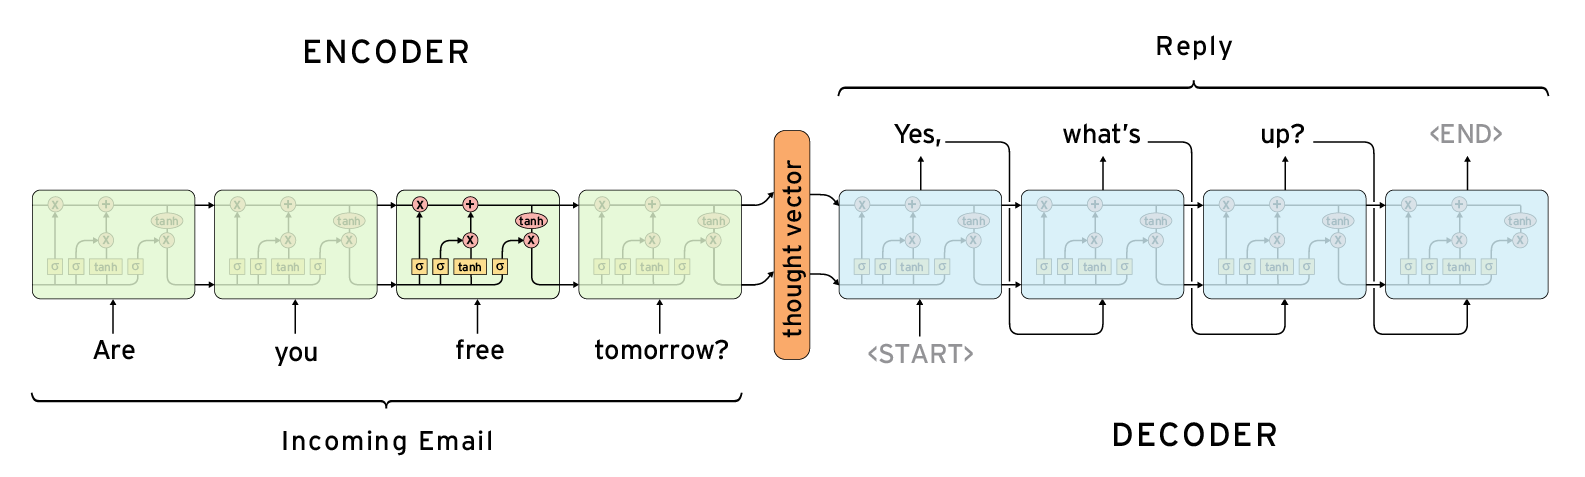
\includegraphics[width=14cm]{Images/seq2seq.png}
    \caption{A seq2seq model for question answering task. Source: \citep{Britz-2016}}
    \label{fig:seq2seq}
\end{figure} 

We utilized this idea for representing words from our dataset. To receive word representations from an RNN, we first trained it to classify words based on labels by one annotator (we chose $O1$), then for each word we found values of the last hidden state of the RNN and used this vector as features in word understandability detection for different users.

As a direct classifier, we trained a character-level RNN using PyTorch framework\footnote{\url{https://pytorch.org/}} and one GPU Tesla K80. For training we lowercased all words, converted them to a singular form and substituted all Unicode symbols with ASCII analogs.  We tried several RNN architectures and hyperparameter sets; the detailed information is available in Appendix \ref{appx:rnn}. 

We got the best F score macroaveraged (sec. \ref{sec:clf-eval}) on three classes for the RNN with two unidirectional long short-term memory (LSTM) units (described in \ref{sec:lstm}), each with 50 hidden units. The dropout of the model is 0.7. The input size is 57 as the number of unique characters in lowercase and converted to ASCII input words. The output size is 3 as this is the number of classes in our data.

This model reached the best performance on the eighth epoch with $F1= 78.94$ and $accuracy = 81.21\%$ on development set. Using this model we received 50-dimensional word representations which we called FrnnMUTE (French RNN Medical Understandability Text Embeddings). 


\section{Cross-validation scenarios}
For a thorough study of generalization abilities of the developed in this work classification models, we propose to consider three distinct cross-validation scenarios based on different combinations of users and vocabulary in train and test sets (fig. \ref{fig:experiments-description}).

\begin{figure}[h]
    \centering
    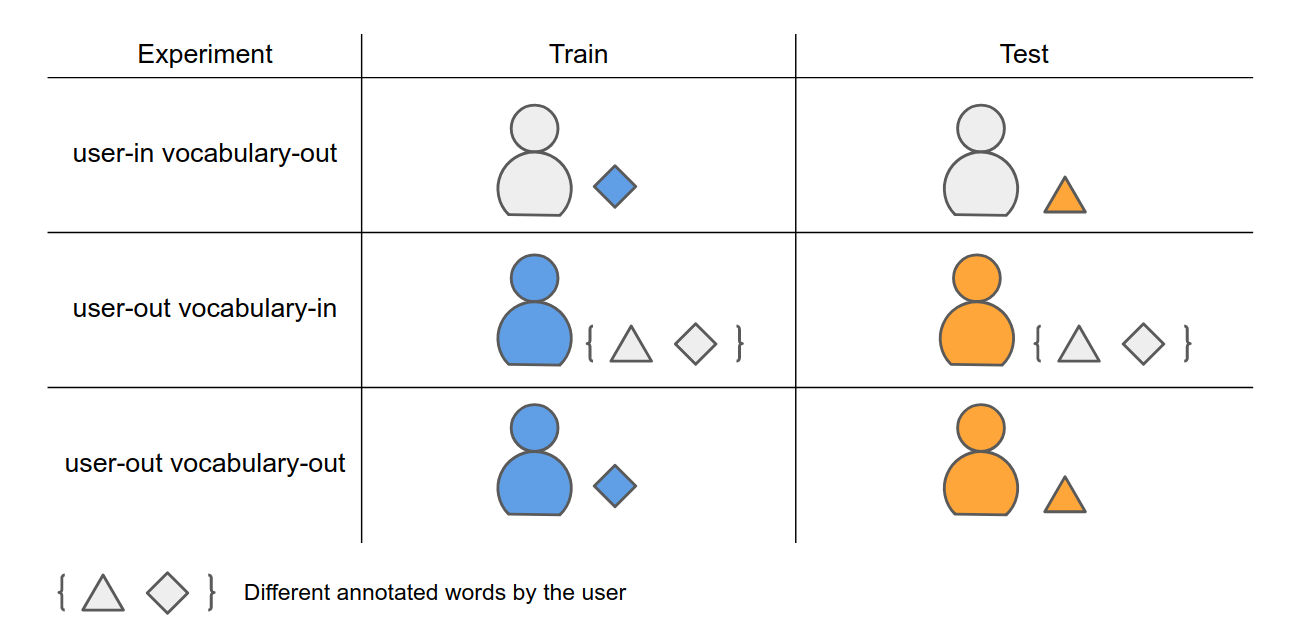
\includegraphics[width=14cm]{Images/Experiments.png}
    \caption{Visual description of the cross-validation experiments. There are experiment types by rows. By columns, there are combinations of a user (annotator) and a set of vocabulary used during training and testing. A user is depicted as a human icon. Different colors of human icons in columns mean that different users were used on training and testing stages. Different shapes of geometrical figures depict subsets of vocabulary. The logic for colors is the same as for human icons.}
    \label{fig:experiments-description}
\end{figure} 

\begin{enumerate}
    \item \textbf{User-in vocabulary-out cross-validation.} This type of experiment follows the scenario from the paper that we are comparing the results with throughout this work \citep{Grabar-PITR2014}.  The cross-validation is done on each dataset (i.e., each user's annotation) separately. The goal of these experiments is to measure the ability of the method (classification model) to generalize class recognition on the \textit{known user} and his known manner to annotate words (that is, his understanding of the meaning of medical words) for \textit{unknown words}.  From the practical perspective, \textit{user-in} means learning the profile of a user. So a model trained by such scenario represents the words understanding or knowledge of the annotator.
      
    \item \textbf{User-out vocabulary-in cross-validation.} In this experiment, we learn from all the annotations of one user and then test the model on annotations of another user. Thereby, in such a setting, we measure the ability of the classifier to generalize on all known words, but for unknown users. This scenario is realistic to a real-world situation: the reference annotations can be obtained only from a couple of users, presumably representing the overall population, but not from all the possible users. Yet, it is necessary to predict the familiarity of medical words for all the potential users even if they did not participate in the annotations. In this scenario, the model learns the profile of a user, and we want to identify whether a new user has the same profile as an another. If the model predicts well for a new user, then it can be used for the identification of incomprehensible words for the new user. 
      
    \item \textbf{User-out vocabulary-out cross-validation.} In this experiment, we use (k-1) folds of data annotated by one user for training and test on the k-th fold of data with annotations by the other user. In this case, we measure the ability of the method to generalize both on \textit{unknown users} and \textit{ unknown vocabulary}. This experiment should be helpful in identifying the number of words needed for determining whether the profile of one user is the same as another in case the model shows good performance.
\end{enumerate}

\bigskip
In this chapter, we introduced the methods which are tested in the experiments in the next chapter. Concretely, we explain our idea of using pre-trained FastText word embeddings for the detection of word difficulty. Also, we describe the process of receiving the novel FrnnMUTE embeddings. Finally, we introduce the three cross-validation scenarios which we will consider during experiments and which go beyond the standard cross-validation described in section \ref{sec:cross-val}. 